\section*{Parte 3}

En esta sección se analizaron señales de AM. Estas señales vienen dadas por:

\begin{equation}
\begin{aligned}
S_{AM}(t) = A_P (1+ m\cdot S_M(t))cos(2\pi f_P t)
\qquad\qquad
S_M(t)= cos(2 \pi f_M t)
\end{aligned}
\label{eq:coeficientrectangular}
\end{equation}

Donde $S_M$ es la que transporta la señal, m es el coeficiente de modulación, $f_p$ es la frecuencia de la portadora, $f_M$ la frecuencia de la moduladora. \par

Luego repitiendo el análisis realizado en la parte 2, se puede observar que en el dominio de la frecuencia, esta formado por 3 deltas ubicados en $f_P-f_M$, $f_P$ y $f_P + f_M$. En particular para las frecuencias dadas, se debe observar 3 picos es $1MHz$, $1,25MHz$ y $1,5MHz$. \par

\begin{figure}[H]
    \centering

    %-------------------------
    %   FIGURA 1
    %-------------------------
    \begin{minipage}[b]{0.45\textwidth}
    \centering
    
\includegraphics[width=0.8\textwidth]{FOTOS_TP6/PARTE 3/parte a/IMG_8326.jpeg}
    \caption{Salida de la señal AM con $f_p=1,25MHz$, $f_M=250kHz$, m =0.5}
    \label{fig:AMa}


    \end{minipage}
    \hfill
    %-------------------------
    %   FIGURA 2
    %-------------------------
    \begin{minipage}[b]{0.45\textwidth}
         \centering
    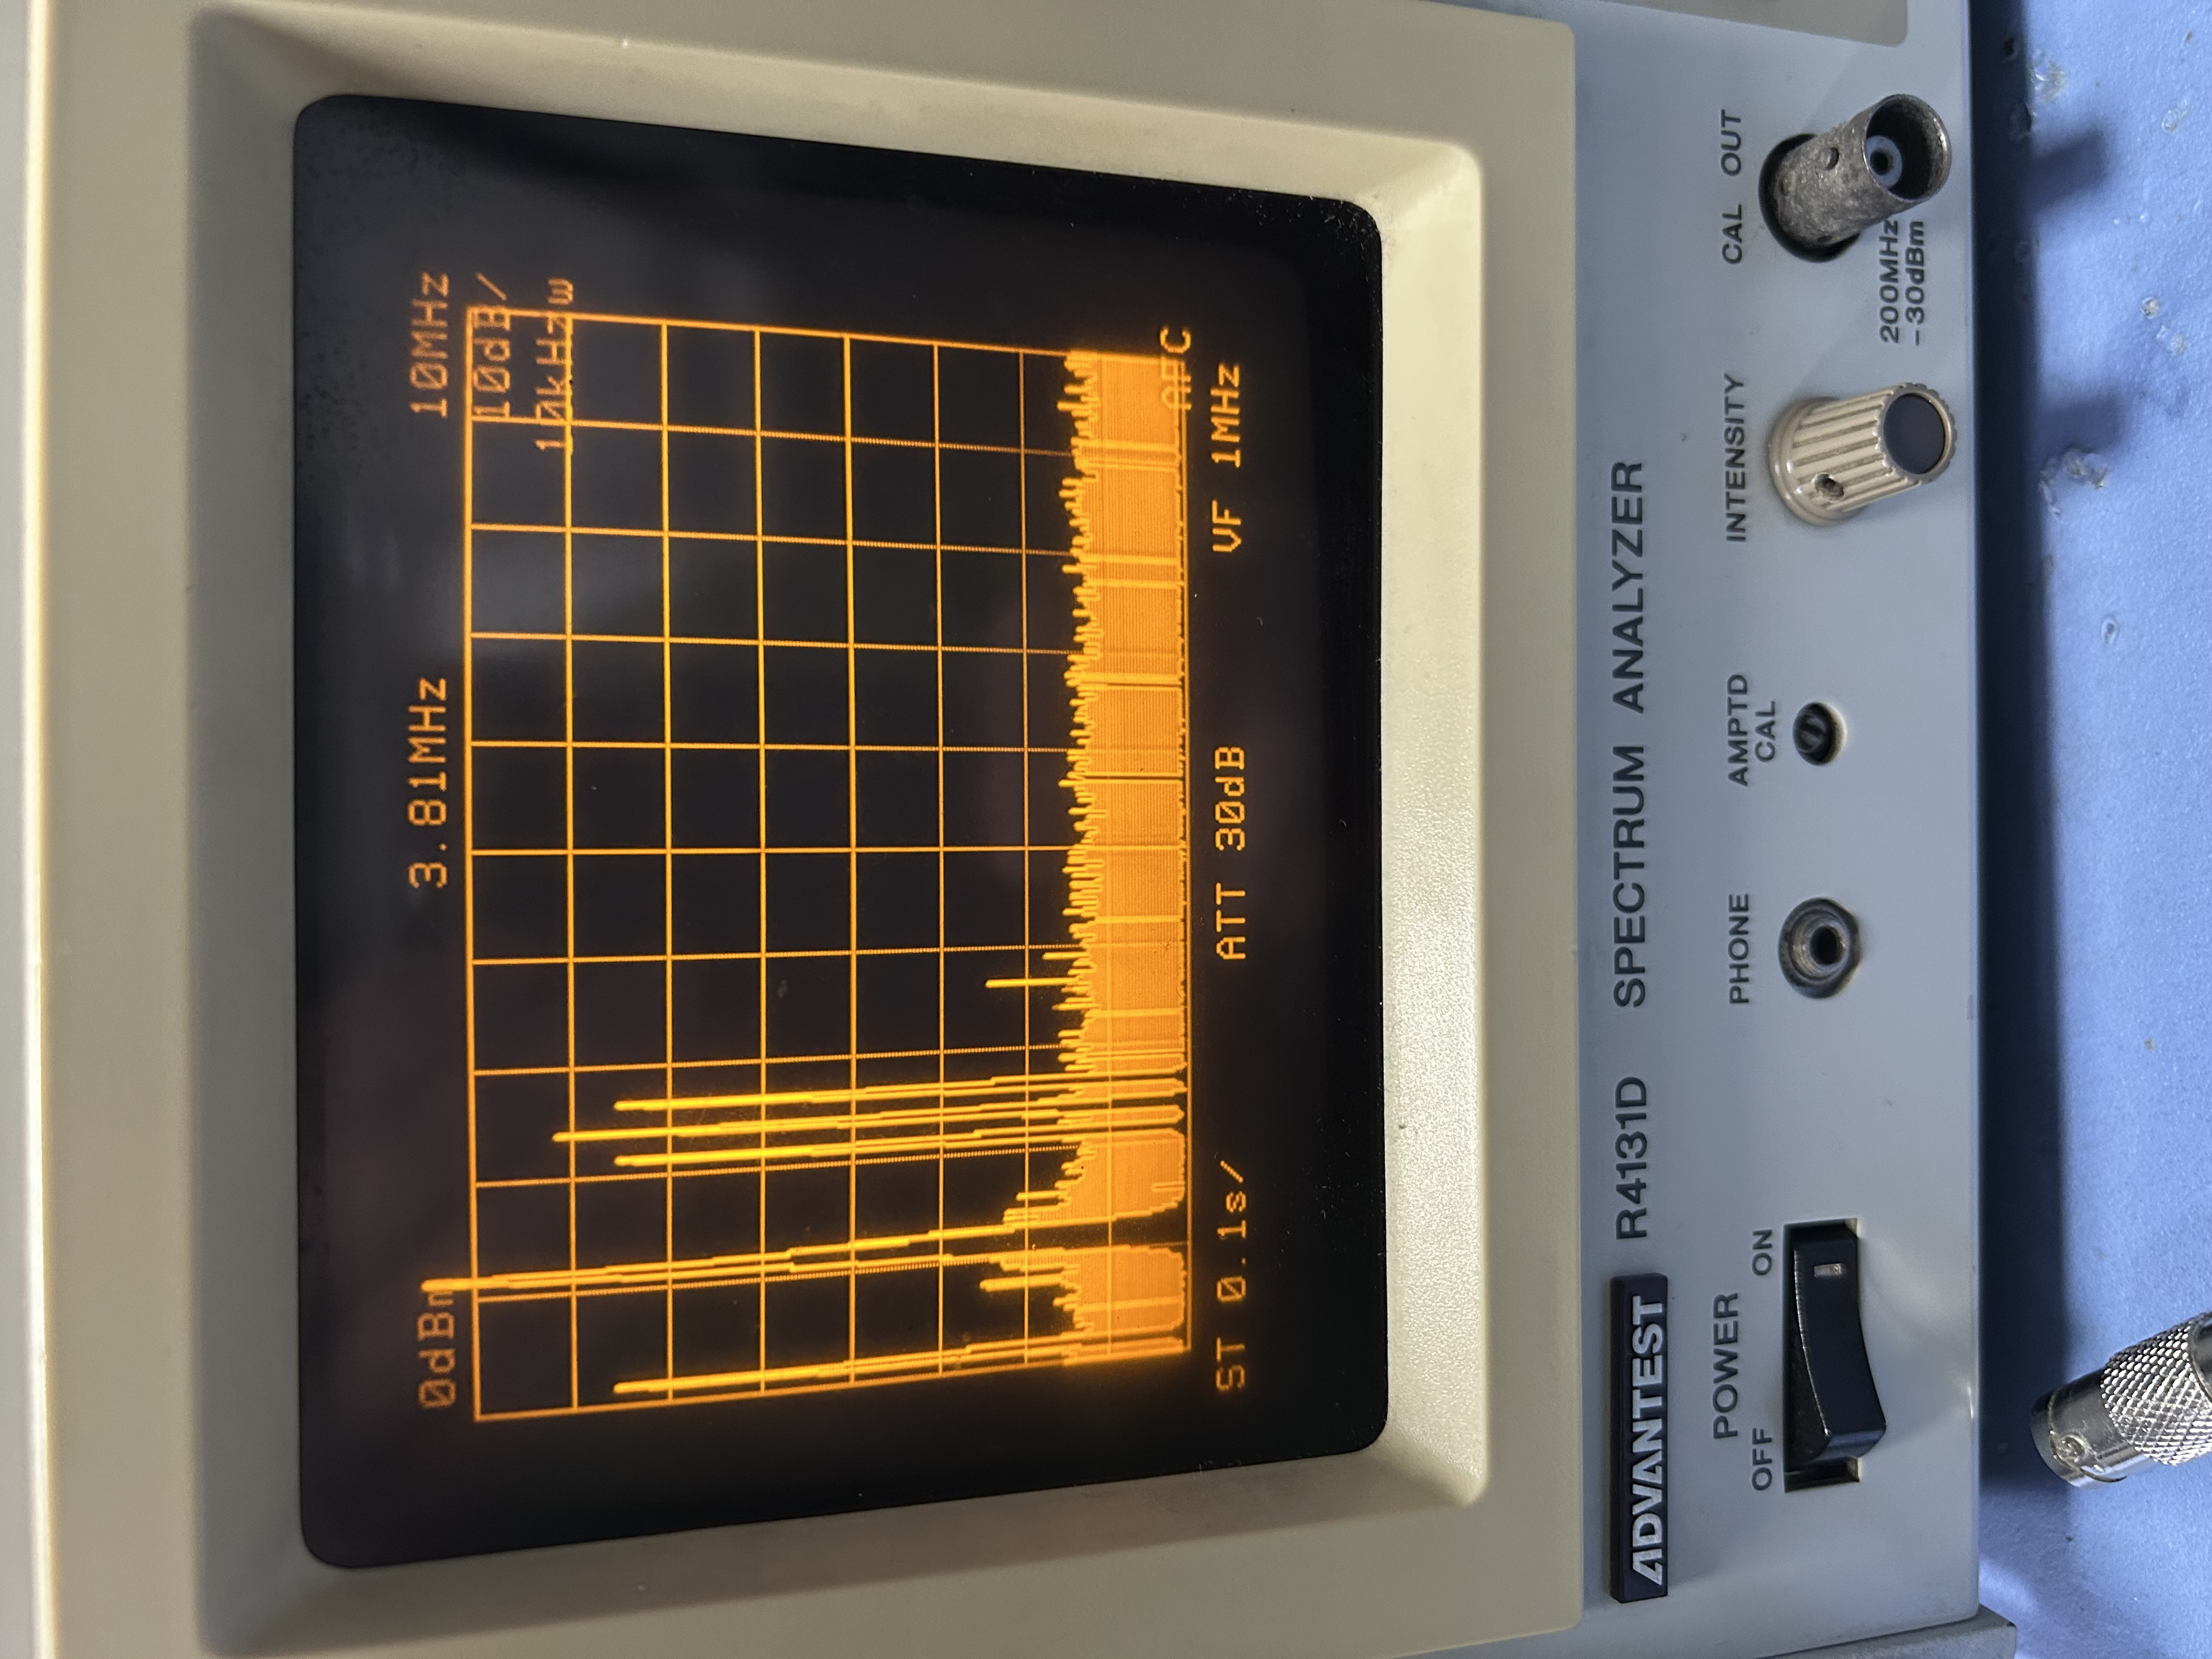
\includegraphics[width=0.8\textwidth]{FOTOS_TP6/PARTE 3/parte b/IMG_8328.jpeg}
    \caption{Salida de la señal AM con $f_p=1,25MHz$, $f_M=250kHz$, m =1}
    \label{fig:AMb}
        \end{minipage}
\end{figure}
\par

Al observar la salida de la señal a y b (observar figuras \ref{fig:AMa} y \ref{fig:AMb}), se puede observar que concuerda con la salida esperada, puesto a que se observan los picos en $1MHz$, $1,25MHz$ y $1,5MHz$. Luego, se puede observar que al aumentar el índice de modulación, los picos no centrales aumentan de magnitud mientras que el central se mantuvo constante. Esto se debe a que haciendo el desarrollo matemático de la señal se observa que los coeficientes de amplitud terminan siendo $A_P$ para el pico central y $\frac{A_P \cdot m}{2}$ para los laterales. Por tal motivo, al aumentar el indice, el pico central se mantuvo constante mientras que los laterales aumentaron.\par

Luego se midieron dos señales AM con características particulares.\par


\begin{figure}[H]
    \centering

    %-------------------------
    %   FIGURA 1
    %-------------------------
    \begin{minipage}[b]{0.45\textwidth}
    \centering
    
\includegraphics[width=0.8\textwidth]{FOTOS_TP6/PARTE 3/parte c/IMG_8332.jpeg}
    \caption{Salida de la señal AM con modulante triangular con $f_p=1,25MHz$, $f_M=200kHz$, m =1}
    \label{fig:AMc}


    \end{minipage}
    \hfill
    %-------------------------
    %   FIGURA 2
    %-------------------------
    \begin{minipage}[b]{0.45\textwidth}
         \centering
    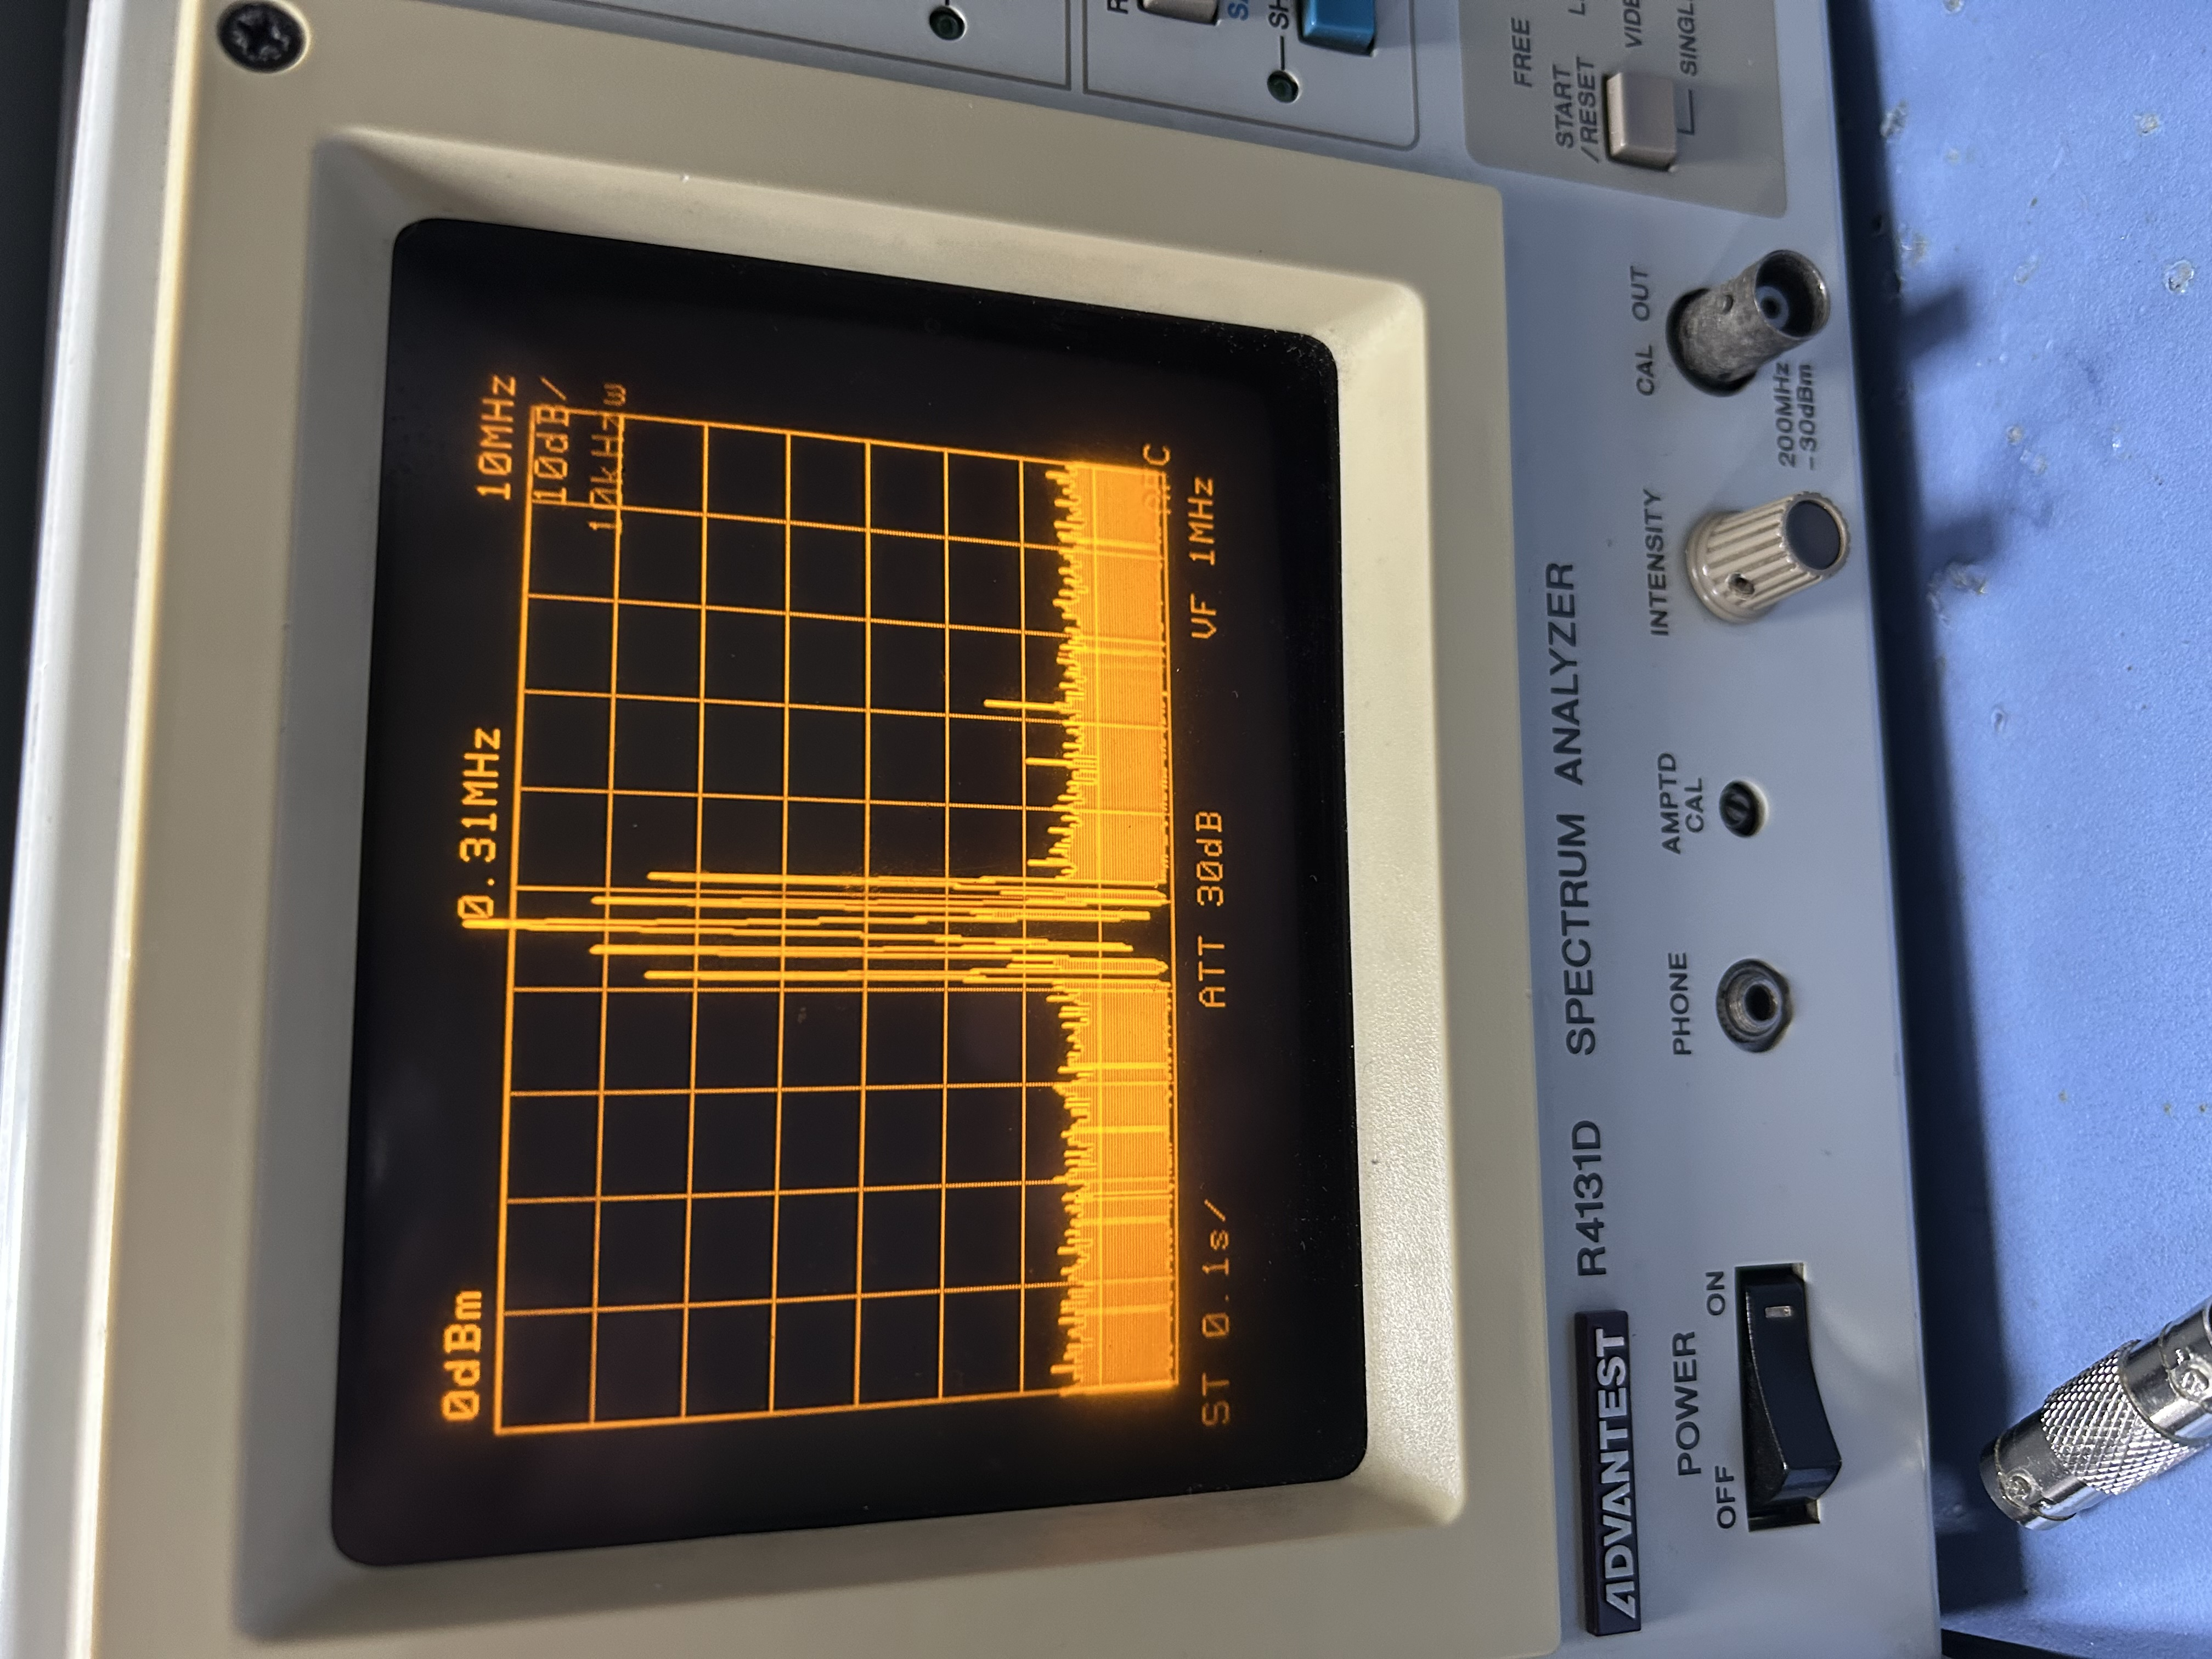
\includegraphics[width=0.8\textwidth]{FOTOS_TP6/PARTE 3/parte d/IMG_8330.jpeg}
    \caption{Salida de la señal AM con $f_p=f_m=250kHz$,  m =1}
    \label{fig:AMd}
        \end{minipage}
\end{figure}
\par

La primera fue una señal modulada por una señal triangular de frecuencia $f_P=1,25MHz$ y $f_m = 200kHz$. Aquí se usó $f_m =200kHz$ puesto a que el generador no fue capaz de llegar a los 250kHz. Al observar la imagen \ref{fig:AMc}, se puede observar lo siguiente: \par
Se observó un pico principal de la portadora a una frecuencia de $f=1,25MHz$, lo cual concuerda con la teoría según la ecuación descripta anteriormente de una señal AM. Por otra parte, a diferencia de el caso de una modulante senoidal, aquí se ven más armónicos aparte de $f_P-f_M$, $f_P$ y $f_P + f_M$. Puesto a lo deducido en la parte 2, una señal triangular puede ser descripta por una serie de fourier con armónicos impares. Luego, al observar los armónicos, se observan amónicos de la forma $f_P-n\cdot f_M$, $f_P$ y $f_P + n \cdot f_M$ con n impar. Los otros picos que no cumplen esta fórmula pueden considerarse ruido que no forma parte de la señal y pudo haber sido eliminado aumentando el atenuador.\par

Finalmente, se estudió una señal senoidal de misma frecuencia modulante y portadora. Al observar la figura \ref{fig:AMd}, se pudo observar una gran correlación con lo aproximado teóricamente, puesto a que según la fórmula ya mencionada, se debían observar picos en $f=0$ $f=250kHz$ y en $f=500kHz$. En particular el pico en la $f=0$ fue tapado por el nivel de continua. Luego, lo visto del otro lado del nivel de continua se debe a que al trabajar con señales reales, el espectro es simétrico respecto del origen de coordenadas.


